\documentclass{article}
\usepackage[utf8]{inputenc}
\usepackage{amsmath, amssymb, amsthm}
\usepackage{float}

\usepackage{listings}
\usepackage{xcolor}

\usepackage{tikz}
\usepackage{float}

\theoremstyle{definition}
\newtheorem{rules}{Rule}[section]
\newtheorem{definition}[rules]{Definition}
\newtheorem{remark}[rules]{Remark}
\newtheorem{example}[rules]{Example}

\definecolor{codegreen}{rgb}{0,0.6,0}
\definecolor{codegray}{rgb}{0.5,0.5,0.5}
\definecolor{codepurple}{rgb}{0.58,0,0.82}
\definecolor{backcolour}{rgb}{0.95,0.95,0.92}

\lstdefinestyle{thestyle}{
    backgroundcolor=\color{backcolour},
    basicstyle=\ttfamily\footnotesize,
    keywordstyle=\color{red!80}\bfseries,
    ndkeywordstyle=\color{blue!80}\bfseries,
    identifierstyle=\color{black},
    commentstyle=\color{codegreen},
    stringstyle=\color{codepurple},
    breakatwhitespace=false,
    breaklines=true,
    captionpos=b,
    keepspaces=true,
    numberstyle=\tiny\color{codegray},
    numbers=left,
    numbersep=2pt,
    showspaces=false,
    showstringspaces=false,
    showtabs=false,          
    tabsize=2
}

\lstset{style=thestyle}

\lstdefinelanguage{TML}{ 
    keywords={changeto, move, goto, if, while, module, accept, reject, halt, alphabet},
    ndkeywords={left, right, blank},
    sensitive=true,
    comment=[l]{//},
    morecomment=[s]{/*}{*/},
    morestring=[b]',
    morestring=[b]"
}

\title{TML Specification}
\author{Pete Gautam}

\begin{document}
    \maketitle

    In this document, we will define the syntax of the TML, starting with an example. We next analyse the syntax and define execution of a valid TML program on a tape in a similar manner to the execution of a TM.

    Consider the following TML program.
\begin{lstlisting}[language=TML]
// checks whether a binary number is divisible by 2
alphabet = {0, 1}
module isDiv2 {
    // move to the end
    while 0, 1 {
        move right
    } if blank {
        move left
        // check last letter is 0
        if 0 {
            accept
        } if 1, blank {
            reject
        }
    }
}
\end{lstlisting}
    A program in TML is used to execute on a tape, so the syntax used guides us in executing the program on a tape. 
    \begin{itemize}
        \item A valid TML \emph{program} is composed of an \emph{alphabet}, followed by one or more \emph{modules}. In the example above, the alphabet of the program is $\{0, 1\}$, and the program has a single module called \texttt{isEven}.
        \item A module contains one or more \emph{blocks} (a specific sequence of commands). There are two types of blocks- \emph{basic blocks} and \emph{switch blocks}.
        \item A basic block consists of \emph{basic commands} (\textit{changeto}, \textit{move} or \textit{flow} command). A basic block consists of at least one basic command, but it is not necessary for a basic block to be composed of all the basic commands. If multiple commands are present in a basic block, they must be in the following order- \textit{changeto}, \textit{move} and \textit{flow} command. In the program above, there is are many basic blocks, e.g. at lines 4, 6, 8-9 and 11-12. We do not say that line 8 is a basic block by itself; we want the basic block to be as long as possible.
        \item A \emph{switch block} consists of cases (\textit{if} or \textit{while} commands), each of which corresponds to one or more letters. A switch block must contain precisely one case for each of the letter in the alphabet, including the \texttt{blank} letter. The first block within a case block cannot be another switch block. In the program above, there is a switch block at lines 3-14 and a nested switch block at lines 7-13.
        \item The body of an \textit{if} command can be composed of multiple blocks. These blocks can be both basic blocks and switch blocks. We can see this at lines 5-13; the \textit{if} block has a basic block at line 6 and then a switch block.
        \item The body of a \textit{while} command must be composed of a single basic block. The basic block cannot have a \textit{flow} command. This is because when we execute a \textit{while} block, the next block to run is the switch block it is in; we cannot accept, reject or go to another module.
        \item A switch block must be the final block present; it cannot be followed by a basic block.
    \end{itemize}
    
    \begin{figure}[htb]
        \centering
        \begin{align*}
            \textit{program} &= \textit{alphabet} \ \textit{module}^+ \\
            \textit{alphabet} &= \texttt{alphabet} \ \texttt{=} \ \texttt{\{} \ \textit{seq-val} \ \texttt{\}} \\
            \textit{module} &= \texttt{module} \ \textit{id} \ \texttt{\{} \ \textit{block}^+ \ \texttt{\}} \\
            \textit{block} &= \textit{basic-block} \ | \ \textit{switch-block} \\
            \textit{switch-block} &= \textit{case-block}^+ \\
            \textit{case-block} &= \textit{if-block} \ | \ \textit{while-block} \\
            \textit{if-block} &= \texttt{if} \ \textit{seq-val} \ \texttt{\{} \textit{block}^+ \texttt{\}} \\
            \textit{while-block} &= \texttt{while} \ \textit{seq-val} \ \texttt{\{} \ \textit{core-com}^+ \ \texttt{\}} \\
            \textit{basic-block} &= (\textit{core-com} \ | \ \textit{flow-com})^+ \\
            \textit{core-com} &= \texttt{move} \ \textit{direction} \ | \ \texttt{changeto} \ \textit{value} \\
            \textit{flow-com} &= \texttt{goto} \ \textit{id} \ | \ \textit{terminate} \\
            \textit{terminate} &= \texttt{reject} \ | \ \texttt{accept} \\
            \textit{direction} &= \texttt{left} \ | \ \texttt{right} \\
            \textit{seq-val} &= (\textit{value} \texttt{,})^* \ \textit{value} \\
            \textit{value} &= \texttt{blank} \ | \ \texttt{a} \ | \ \texttt{b} \ | \ \texttt{c} \ | \ \dots \ | \ \texttt{z} \ | \ \texttt{0} \ | \ \texttt{1} \ | \ \dots \ | \ \texttt{9} \\
            \textit{id} &= (\texttt{a} \ | \ \texttt{b} \ | \ \texttt{c} \ | \ \dots \ | \ \texttt{z} \ | \ \texttt{A} \ | \ \texttt{B} \ | \ \texttt{C} \ | \ \dots \ | \ \texttt{Z})^+
        \end{align*}
        \caption{The EBNF of the TML.}
        \label{fig:tml_ebnf}
    \end{figure}
    
    The EBNF of the TML is Figure \ref{fig:tml_ebnf}.
    
    We will now consider how to execute a tape on a valid TML program. Let $P$ be a TML program with alphabet $\Sigma$ and let $T$ be a tape on $\Sigma$. We execute $P$ on $T$ inductively, as follows:
    \begin{itemize}
        \item At any point during execution, we maintain 3 objects- a tape on $\Sigma$, a block of $P$ and the tapehead index. 
        \item At the start, the tape is $T$; the tapehead index is $0$; and the block is the first block in the first module in $P$. 
        \item At some point during the execution, assume that we have the tape $S$, tapehead index $j$, with tapehead value $T(j) = t$, and a block $b$. We define the next triple as follows:
        \begin{itemize}
            \item if $b$ is a \textit{switch} block, we take the first block from the case corresponding to the tapehead value- because the program is valid, this is a basic block; we will now refer to this block as $b$.
            \item if $b$ has a \textit{changeto} \texttt{val} command, the next tape $T'$ is given by 
            \[T'(x) = \begin{cases}
                \texttt{val} & x = i \\
                T(x) & \text{otherwise}.
            \end{cases}\]
            If the \textit{changeto} command is missing, then the tapehead $T' = T$.
            \item if $b$ has a \textit{move} \texttt{dir} command, the next tapehead index is given by:
            \[i' = \begin{cases}
                i+1 & \texttt{dir} = \texttt{right} \\
                i-1 & \texttt{dir} = \texttt{left}.
            \end{cases}\]
            If the \textit{move} command is missing, then $i' = i-1$.
            \item we either terminate or determine the next block $b'$ to execute (in decreasing precedence):
            \begin{itemize}
                \item if the block is the body of a while case block, then the next block $b' = b$, i.e. we execute this switch block again (not necessarily the same case block);
                \item if the block contains a terminating \textit{flow} command, execution is terminated and we return the terminated state (\texttt{accept} or \texttt{reject});
                \item if the block contains a \textit{goto} \texttt{mod} command, then $b'$ is the first block of the module \texttt{mod};
                \item if the block is not the final block in the current module, then $b'$ is next block in this module;
                \item otherwise, execution is terminated and we return the state \texttt{reject}.
            \end{itemize}
        \end{itemize}
        If execution is not terminated, execution continues with the next triplet.
    \end{itemize}
    
    \begin{figure}[htb]
        \centering
        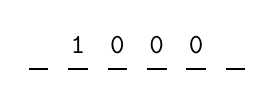
\begin{tikzpicture}
            \foreach \x[count=\i] in {, 1, 0, 0, 0, } {
                \draw[thick] (\i*0.5-0.25, 0) -- (\i*0.5, 0);
                \node at (\i*0.5-0.125, 0.3) {\texttt{\x}};
            }
        \end{tikzpicture}
        \caption{A TM tape on $\{0, 1\}$.}
        \label{fig:tml_tape_example}
    \end{figure}
     
    We will now illustrate this process. We execute the program \texttt{isEven} on the tape at Figure \ref{fig:tml_tape_example}.
    \begin{itemize}
        \item Initially, the tape is the given tape; the current block is at lines 5-15; and the tapehead index is $0$, with value $1$.
        
        \item Since the tapehead value is \texttt{1}, the basic block to be executed is lines 5-7. Hence,
        \begin{itemize}
            \item the tape remains unchanged;
            \item the current block is still at lines 5-15; and
            \item and the tapehead index becomes $1$, with value \texttt{0}.
        \end{itemize}
        
        \item The transition for \texttt{0} and \texttt{1} are the same with respect to the current block. This means that we keep moving to the right until we end up at a blank symbol. At that point, the following is the state of the tape:
        \begin{figure}[H]
            \centering
            \begin{tikzpicture}
                \foreach \x[count=\i] in {, 1, 0, 0, 0, } {
                    \draw[thick] (\i*0.5-0.25, 0) -- (\i*0.5, 0);
                    \node at (\i*0.5-0.125, 0.3) {\texttt{\x}};
                }
                \draw[->] (2.875, -0.5) -- (2.875, -0.1);
            \end{tikzpicture}
        \end{figure}
        The arrow points at the tapehead value. We are still executing the same block, and the tape has not been altered.
        
        \item Now, since the tapehead value is \texttt{blank}, we move to the left. Moreover, the current block is at lines 10-14. The tape has still not been changed. The current value is now $0$.
    
        \item The tapehead value is currently \texttt{0}. So,  
        \begin{itemize}
            \item the tape value changes to \texttt{blank};
            \item we have reached the \texttt{accept} command; and
            \item the tapehead pointer move to the left (by default), to index $2$.
        \end{itemize}
        Hence, execution terminates, with result accept and the following tape state:
        \begin{figure}[H]
            \centering
            \begin{tikzpicture}
                \foreach \x[count=\i] in {, 1, 0, 0, , } {
                    \draw[thick] (\i*0.5-0.25, 0) -- (\i*0.5, 0);
                    \node at (\i*0.5-0.125, 0.3) {\texttt{\x}};
                }
                \draw[->] (1.875, -0.5) -- (1.875, -0.1);
            \end{tikzpicture}
        \end{figure}
    \end{itemize}
\end{document}